% LINKS IN STYLE FILE
\documentclass{ueacmpstyle}

% DIFFERENT PACKAGES THAT YOU MAY USE THROUGHOUT YOUR REPORT - LOOK AT OVERLEAF TUTORIALS ON DIFFERENT PACKAGES (i.e. tables)
\RequirePackage{natbib}
\usepackage{graphicx,caption}
\usepackage{appendix}
\usepackage[hyphens]{url}
\usepackage{pdfpages}

\begin{document}
	% HEADER SECTION
	\title{Client Report}    % COURSEWORK TITLE
	% \title{Human Computer Interaction -- Coursework 1} << Example Title
	\author{
		100287756 -- Alfie Arundell-Coote\\
		100287814 -- George Beales\\
		100301701 -- James Wright\\
		% Can just use student number but if you include name separate with double hyphen
		CMP-6045B     % Module code here - use the code that is relevant to you
	}
	\maketitle
	
	\section{Introduction}\label{sec:Intro}
	At a basic level, a food blog website is intended for users to post their meals for other users to see. The complexity can range dramatically, however with more extravagant features then in turn comes more of a chance for a security breach. With our website we have created a simple front end with just the essential features, this means that we can maximise the security potential for our site.
	
	We have two main objectives with this site: the first is making it easy to use so that any user of any level can utilise our site. Our second objective is to ensure that our website is watertight and safe from a multitude of potential cyber attacks.
	In order to complete our first objective we have decided to utilise white space to our advantage by not crowding our site with unnecessary colours, images or buttons. For example our navigation bar only has 3 buttons and a search bar as we felt like if we added much more it could confuse some users.
	
	Our second goal is achieved via implementing certain mitigation's in order to counter security vulnerabilities which are: account enumeration \cite{accenum}, session hijacking \cite{sessionhijack}, SQL injection \cite{sqlinjection}, cross-site scripting \cite{xss} and cross-site request forgery \cite{csrf}. We believe these to be the main 5 common vulnerabilities that could be abused in our site. These security mitigation's do not affect the usability, for example our cookies expire after one hour so that if the user quickly clicks off of the site, they can get back online without the needs to generate new cookies.
	
	\section{How ethics are essential to secure web development}
	
	When creating a secure website there are ethics that come into play. Having secure encryption is ideal so that people's data is safe and secure and not liable to theft from malicious sources. A downside to encryption is that since everything is encrypted, if anything malicious is to take place on our site, it could be very difficult to actually find the malicious people in question. We however did come to the conclusion that we need to focus on the user, as our product is designed for them and by protecting them, we believe this to be the ethical approach.  We also make use of a system administrator who can delete posts that may be inappropriate.
	
	Ethics come into play in other scenarios such a data breach. Companies can be faced with the conundrum that if there is a breach, do they either tell the users immediately or do they try and mitigate and contain the problem before it spreads. We attempt to do both as we make our users sign up with an email address so in the event of a data leak we can alert them via the use of email.
	
	
	
	\section{What mitigation's were coded for each security vulnerability, and should include
		discussions of pre-built libraries, hashing, encryption, usability etc.}
	
	\subsection{Account enumeration}
	In order to protect against account enumeration is via implementing a captcha system so we can stop quick enumeration of usernames, this means that a malicious user cannot simply use bots to check if a username exists as they would need to verify every time. We do not have a way of telling the user that a username is already taken without exposing its existence as a whole, however we have figured that this is the best response as it does not impact the user too heavily. We do however make sure that the HTTP response time taken for an incorrect password is the same as the time taken for an already taken username. \cite{accenum}
	
	\subsection{Session hijacking}
	
	We parse our sessions in cookies as we believe this solves a lot of the session hijacking possibilities
	For session hijacking we made sure to use the HTTP only tag for all cookies in order to insure they cannot be altered via javascript. In our project we would have ideally utilised HTTPS to force browsers to use TLS protocols, this would have ensured encryption between the user and the server for everything, including cookies. \cite{sessionhijack}
	
	\subsection{SQL Injection}
	
	We have countered against traditional string SQL injection as we use something called MongoDB which utilises a specific data format called BSON where queries are represented as binary data (ones and zeros) so direct injection through a string (text) is not available. There is no SQL code at all, as everything is d-one through a schema, all SQL statements are based on a model which stops a user from injecting SQL as they have no access to the SQL code whatsoever. This is essentially input sanitisation. \cite{sqlinjection}
	
	\subsection{Cross-site scripting}
	
	We implemented a node library called helmet \cite{helmet} which allowed us to use a content security policy. This allowed us to specify where we want the browser to run scripts and also use some built in features of the helmet library. This stops a malicious user from being able to inject HTML into text that the server will serve to the user because the script will not run from places that where we did not specify it could not run in the first place. \cite{xss}
	
	\subsection{Cross-site request forgery }
	
	The use of captcha helps us as the user needs to authorise before confirming important actions (such as login), this prevents cross-site forgery as a malicious user cannot automate a request without authentication from a captcha. All cookies we have implemented cannot be used in cross-site request forgery as they are all unique. We also make use of a secret cookie that retrieves a key from a .env file, utilising .env files means that we do not store sensitive information on our git meaning it cannot be stolen if an attack is to occur. \cite{csrf}
	
	
	\section{What Authentication method/s were coded, and evidence of how they increase both
		usability and security.}
	
	\subsection{2FA}
	
	Hackers do not care if a business is big or small, if it is liable to an easy attack they WILL go for it, this is why we have decided to utilise 2FA (2 factor authentication) when logging in to our site. 2FA halts an attack via the use of bots which essentially rapidly guess passwords against an account as once the password is guessed correctly the user will receive a 5 character code that they then need to input into the site so they can log in. This means that if a hacker would like to gain access to a persons account on our site, they need to also have access to said persons email address which is significantly harder to obtain than just a username and password for our site.
	
	\subsection{Passwords}
	
	Passwords are the base line of defense against unauthorised access to an account. The user can pick their own password, ideally something memorable to them but not anything too specific such as their name or just "password". The stronger the password the more protected the account and therefore the less are the chances for it to be breached.
	
	\subsubsection{Hashing our Passwords}
	
	We have irreversible hashing that means that with our B-crypt \cite{bcrypt} library that if the same word was hashed for a second time it would never be the same. We authenticate passwords via comparing hashes to one another and also utilising a practice called "salting" which encrypts a password even further, we do this 8 times.
	
	\subsection{Captcha}
	
	We have lastly implemented captchas in another bid to halt brute force attacks on our users. Having a captcha present on login prevents the use of bots to rapidly attempt to log in to our site as I mentioned earlier in the 2FA section as it requires the user to verify a number of images before logging in. The second place we have implemented a captcha is in registration, this prevents the use of bots to create a multitude of accounts on our site which could lead to many fake accounts being created and in turn wasting resources.
	
	\section{Discussion and evidence of user testing}
	
	when a post is deleted, the ID of the post gets added to the URL. If the URL was changed before the URL gets checked, the cookie/session is checked to see if the person deleting it has actually made this request.
	
	For our user testing we carried out multiple tests in order to make sure that the core functions of our website worked as well as the key security and authentication features.
	
	
	
	\section{Discussion and evidence of system unit testing}
	
	In this section I will detail the unit tests we carried out to identify bugs.
	The unit tests were carried out using the 'jest' library, which is a module for unit testing, with each test only being able to pass or fail\\
	
	To make our code easy to test, we split up a lot of the code in the routes into functions with return values to test.
	Individual tests were written after each function was designed. The tests are located in the tests folder.\\
	
	The first tests were carried out on auth.routes.js. The functions tested were authFn, encryptpass and authenticateEmail. The goal of the first was to ensure that authFn returns true or false depending on the session it reads. This helps identify any bugs if the session was incorrect.
	The encryption test was mainly to check if the hashing was valid by using compareSync to compare a string and a hash. This was expected to return true. The last test involved the process of sending emails. For this function we had to mock the nodemailer module and then get the results of the mock when calling the method.\\
	
	The second test was carried out on getPosts() in post.routes.js.
	In this test mongoDB had to mocked through the library 'mockingoose'. This means we can get the model to return an element when a particular function is called. The method is called to check for any errors and then we retrieve results from the model, with the assertion that the model has returned the exact same object as our test data.
	
	The final test was on user.routes.js. This checked the user existing method by also mocking mongoDB with test data. The function is then called and the assertion is that it returns true.
	The find operation is then carried out on the model to asser that the result matches our test data. Upon an error in the try/catch loop the test will fail with the message of the error.\\
	
	All these tests can be found in our completed plan document. Our final coverage was 60 percent of lines being tested in the routes folder, 35 percent in the db.js file and 100 percent coverage on all of the models in the models folder.
	
	
	
	\section{Conclusion}\label{sec:Con}
	
	If we had more time I think our main goal would be to secure against more against Cross site request forgery. Even though we believe that our captcha stops most rouge requests we believe it would be more beneficial to add csrf tokens to all our forms and make sure that every form that is submitted to the server contains the correct tokens in order to submit properly. 
	
	We definitely could improve on our authentication by adding another layer or even an easier and more secure layer such as using a mobile device's authentication app. This would be easier for the users to use and adds a physical level or security as you would need to have access to a singular mobile device.
	
	Overall we believe that our food blog website would rate very well for security as we had designed our system from the ground up to be resistant to the most common forms of attacks that hackers would try. The fact that it is a blog website defines our security to be much less than say, a banking website but, any website that uses accounts should take very seriously the impacts of housing user information.
	
	% Setting up your bibliography style - NOTE CMP uses Harvard style so stick with apalike for now
	\bibliographystyle{apalike}
	% Link your bibliography to your main.tex
	\bibliography{myBib.bib}
	% Look at DBLP or Google Scholar for references (NOTE - Google Scholar can produce usable bib entries - allowing you to copy and paste into myBib.bib)
	
	\newpage
	% Following command starts an appendices section (NOTE - You have included appendix as a package at the start of the document)
	\appendix
	
	\section{Appendix}
	
	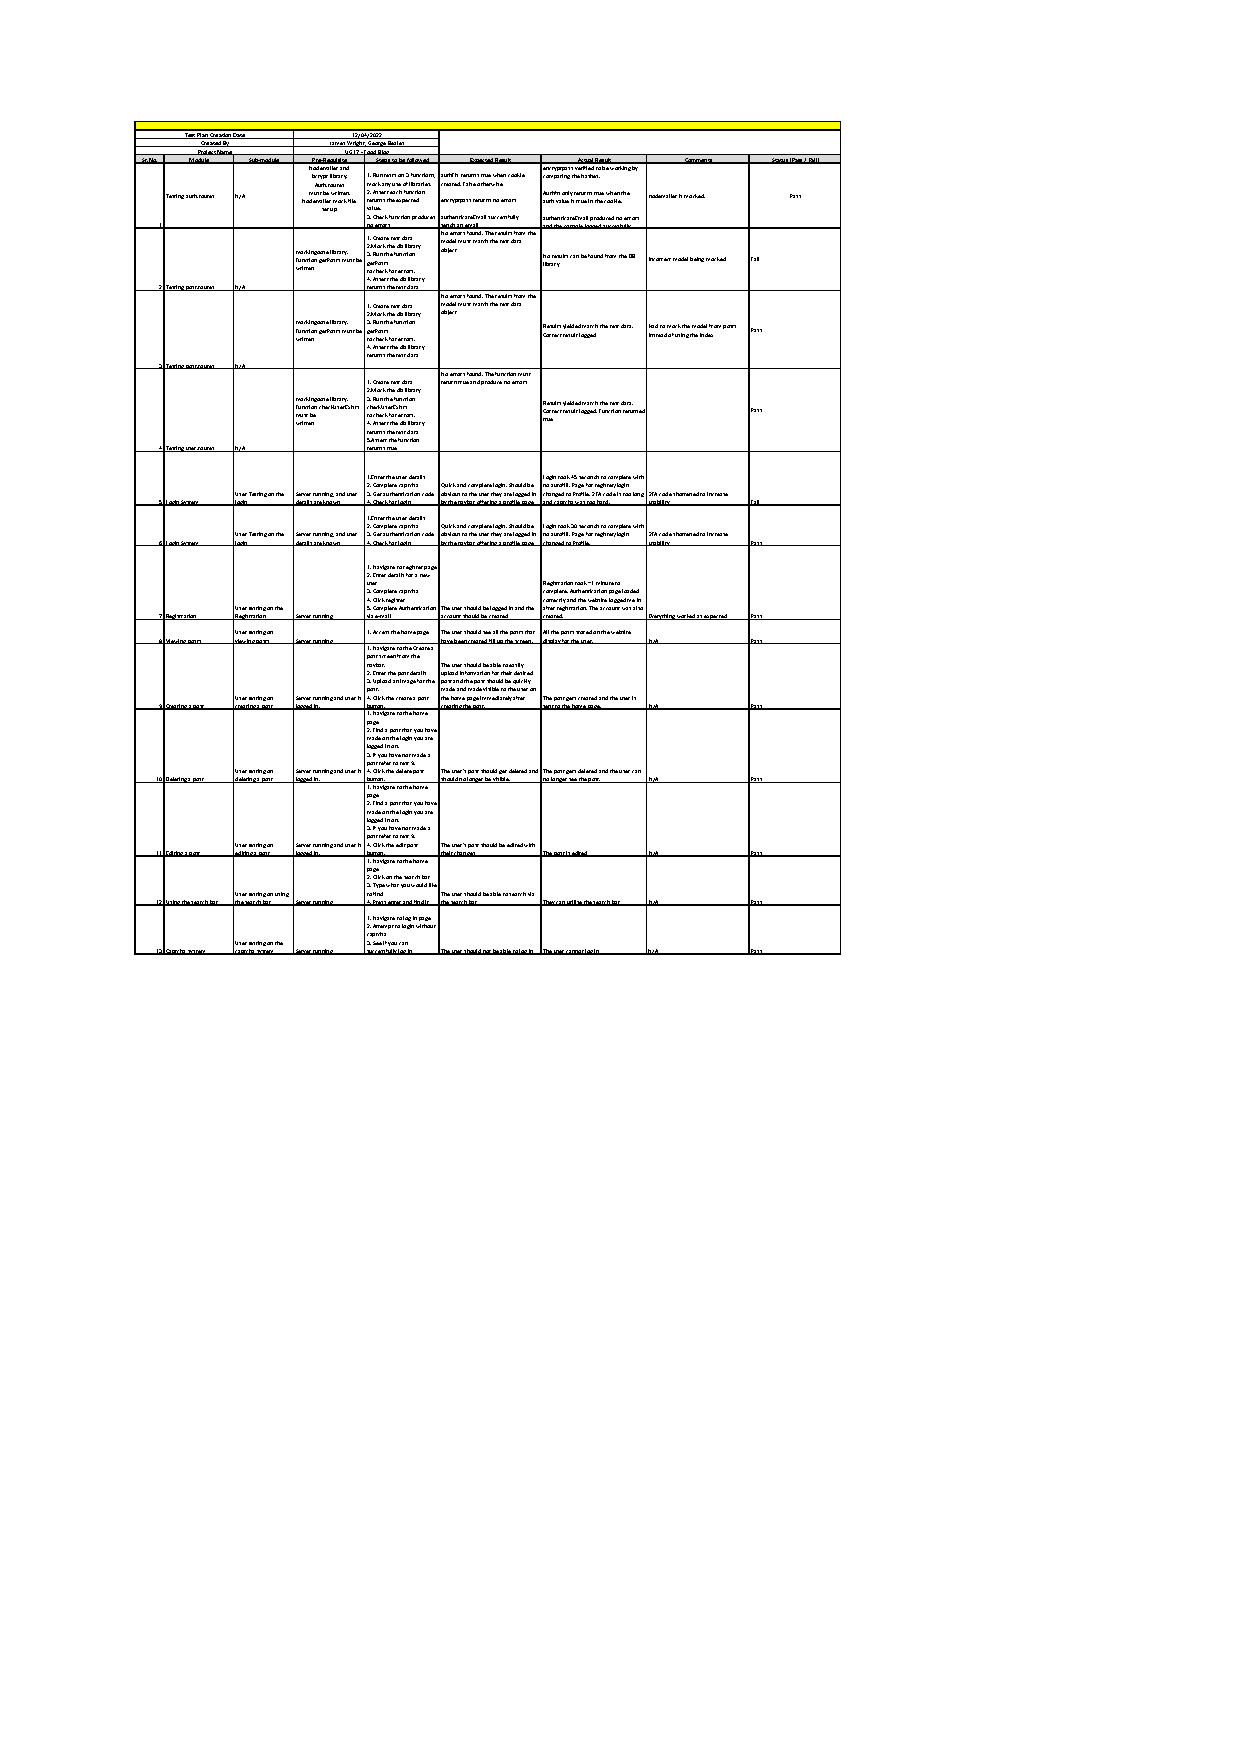
\includepdf[]{testing.pdf}
	
\end{document}
